% https://en.wikipedia.org/wiki/LZ77_and_LZ78
LZ77\cite{doc4} operates on the concept of a sliding window, which tracks a portion of previously processed data. The algorithm identifies the longest match between a substring in the look-ahead buffer and a substring within the sliding window. After locating a match, the window slides forward based on the length of the match.

\begin{figure}[ht]
    \centering
    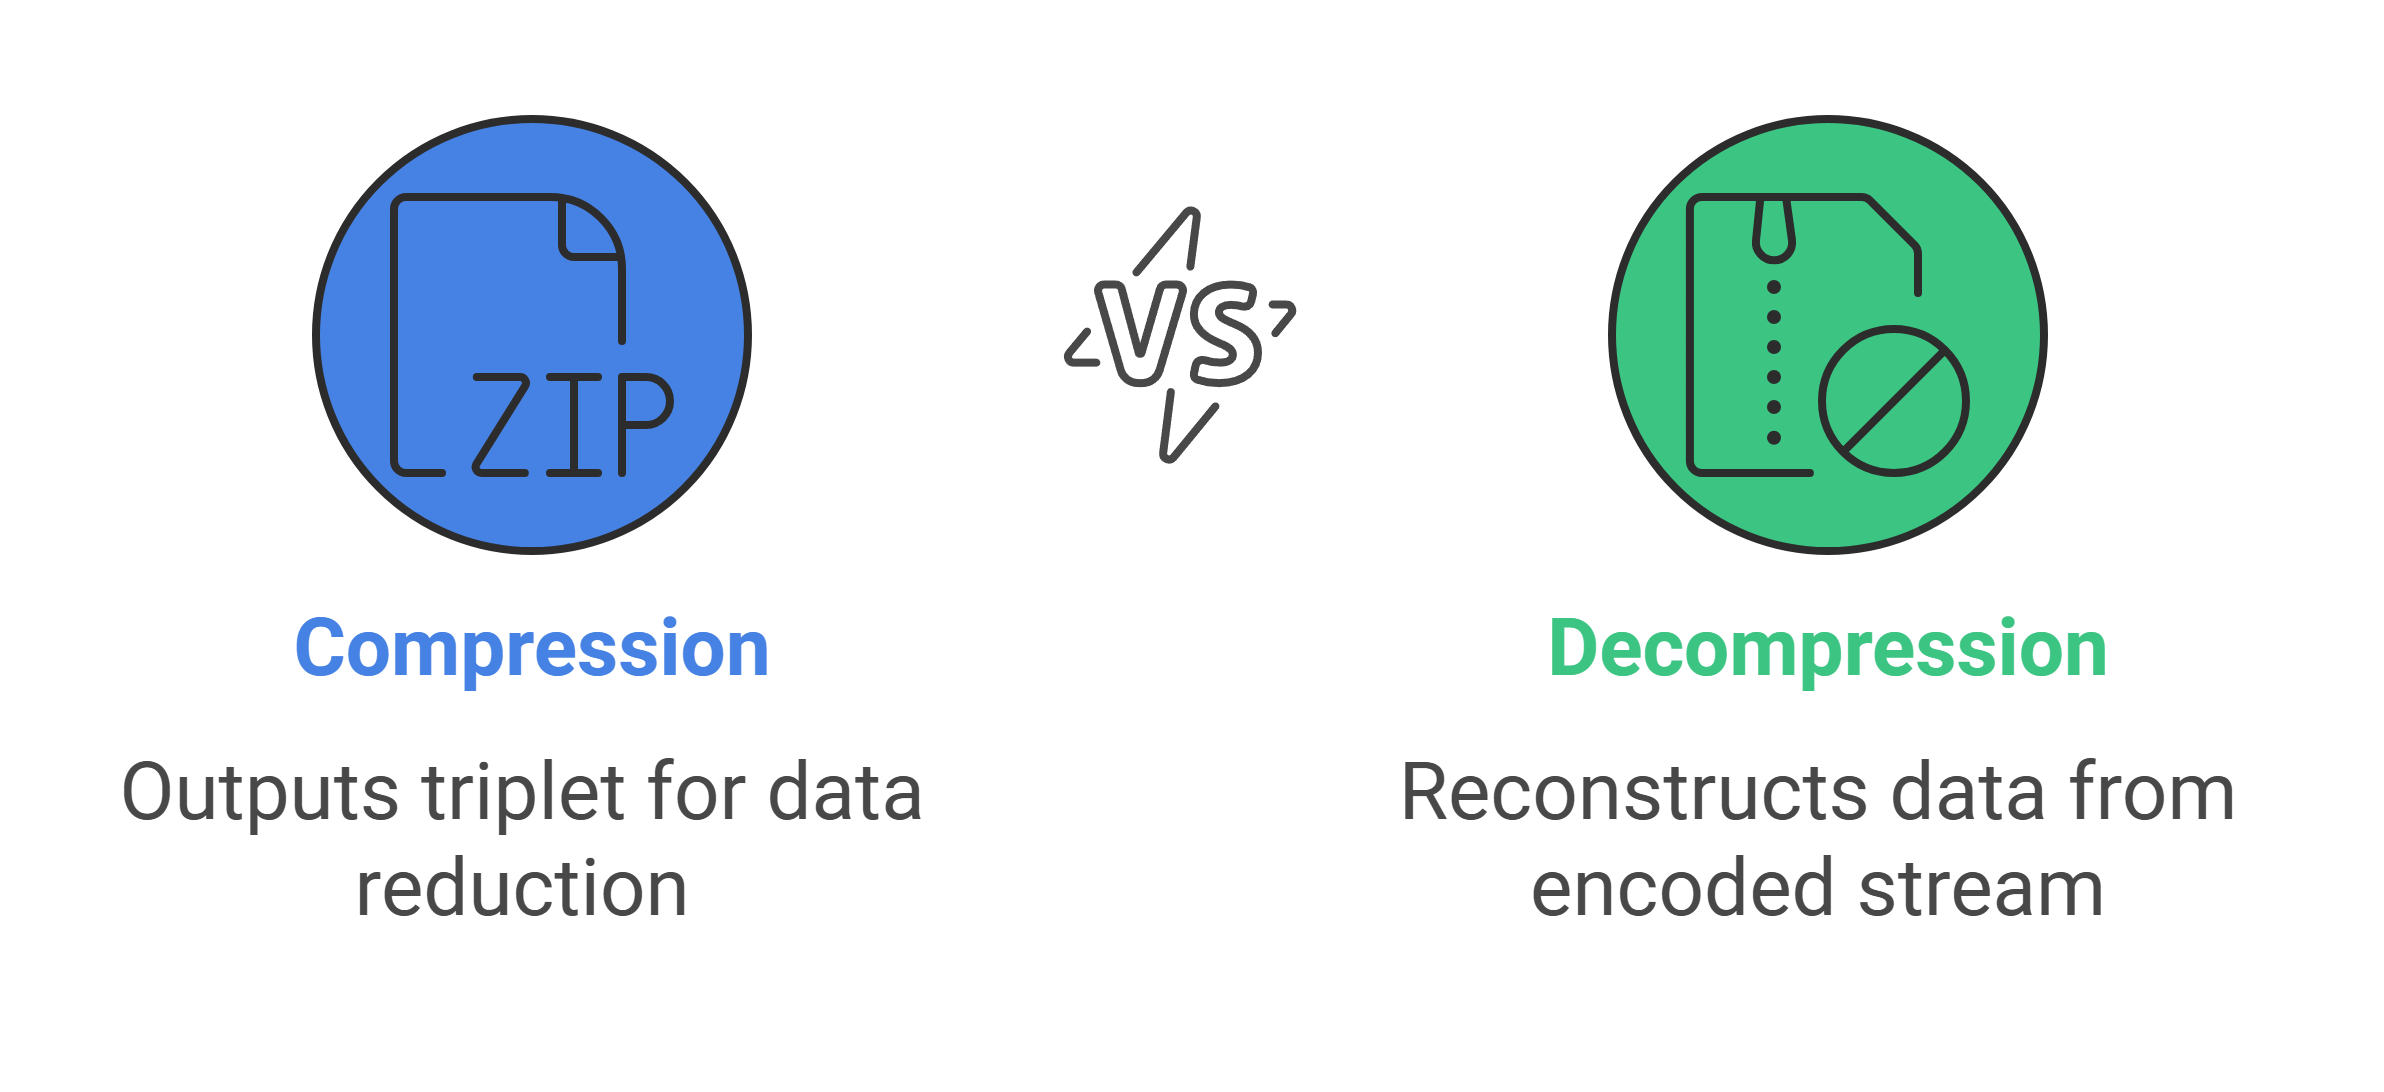
\includegraphics[width=0.8\linewidth]{Figures/LZ77.png}
    \caption{LZ77 Compression and Decompression}
    \label{fig:lz77}
\end{figure}

During compression, the algorithm outputs a triplet: a pointer to the starting position of the match (relative to the start of the sliding window), the length of the match, and the first unmatched character in the look-ahead buffer. If no match is found, the algorithm outputs a null pointer and the unmatched character.

\vspace{10pt}
% The decompression algorithm processes the compressed stream from start to end. For each null pointer, it appends the associated byte directly to the end of the output stream. For each non-null pointer, it reads back to the specified offset from the current end of the output stream and appends the specified number of bytes to the end of the output stream.

For decompression, the process starts by reading the encoded stream sequentially. When a null pointer is encountered, the algorithm appends the corresponding character to the output. For non-null pointers, the algorithm retrieves the matched substring using the pointer and length and then appends the retrieved substring to the output.
